%%%%%%%%%%%%%%%%%%%%%%%%%%%%%%%%%%%%%%%%%%%%%%%%%%%%%%%%%%%%%%%%%%% 
%                                                                 %
%                            CHAPTER                              %
%                                                                 %
%%%%%%%%%%%%%%%%%%%%%%%%%%%%%%%%%%%%%%%%%%%%%%%%%%%%%%%%%%%%%%%%%%% 

\chapter{Information about the thesis}

\begin{description}
   \item[Title:] Counting shells (a more descriptive name is a WIP).
   \item[Subject: ] Develop a vision-algorithm to label and count shells from pictures taken on the Belgian shore.
   \item[Description: ] In march 2018, EOS and VLIZ organised a shell counting day, volunteers were asked to help count shells on our shores. With this data, the amount and types of shells being washed ashore, it's possible to map the diversity of our coast. In this thesis I will be attempting to create a vision algorithm that would simplify the job of the volunteers by automatically labeling and counting the shells in pictures. A large part of the difficulty stems from the fact that many types of shell are visually pretty similar. Difficulty is added by the fact that shells aren't always completely intact and that the shells shouldn't have to be manipulated for the algorithm to work, so different orientations are possible. So, are modern multi-class object detectors performant enough to fit our needs?
   \item[Internal research group: ] EAVISE
   \item[University Promoter and Mentor: ] Toon Goedemé - toon.goedeme@kuleuven.be
   \newpage
   \item[Planning: ] 
   \item[Progress: ] 
   \begin{figure}[h]
 	\centering
 	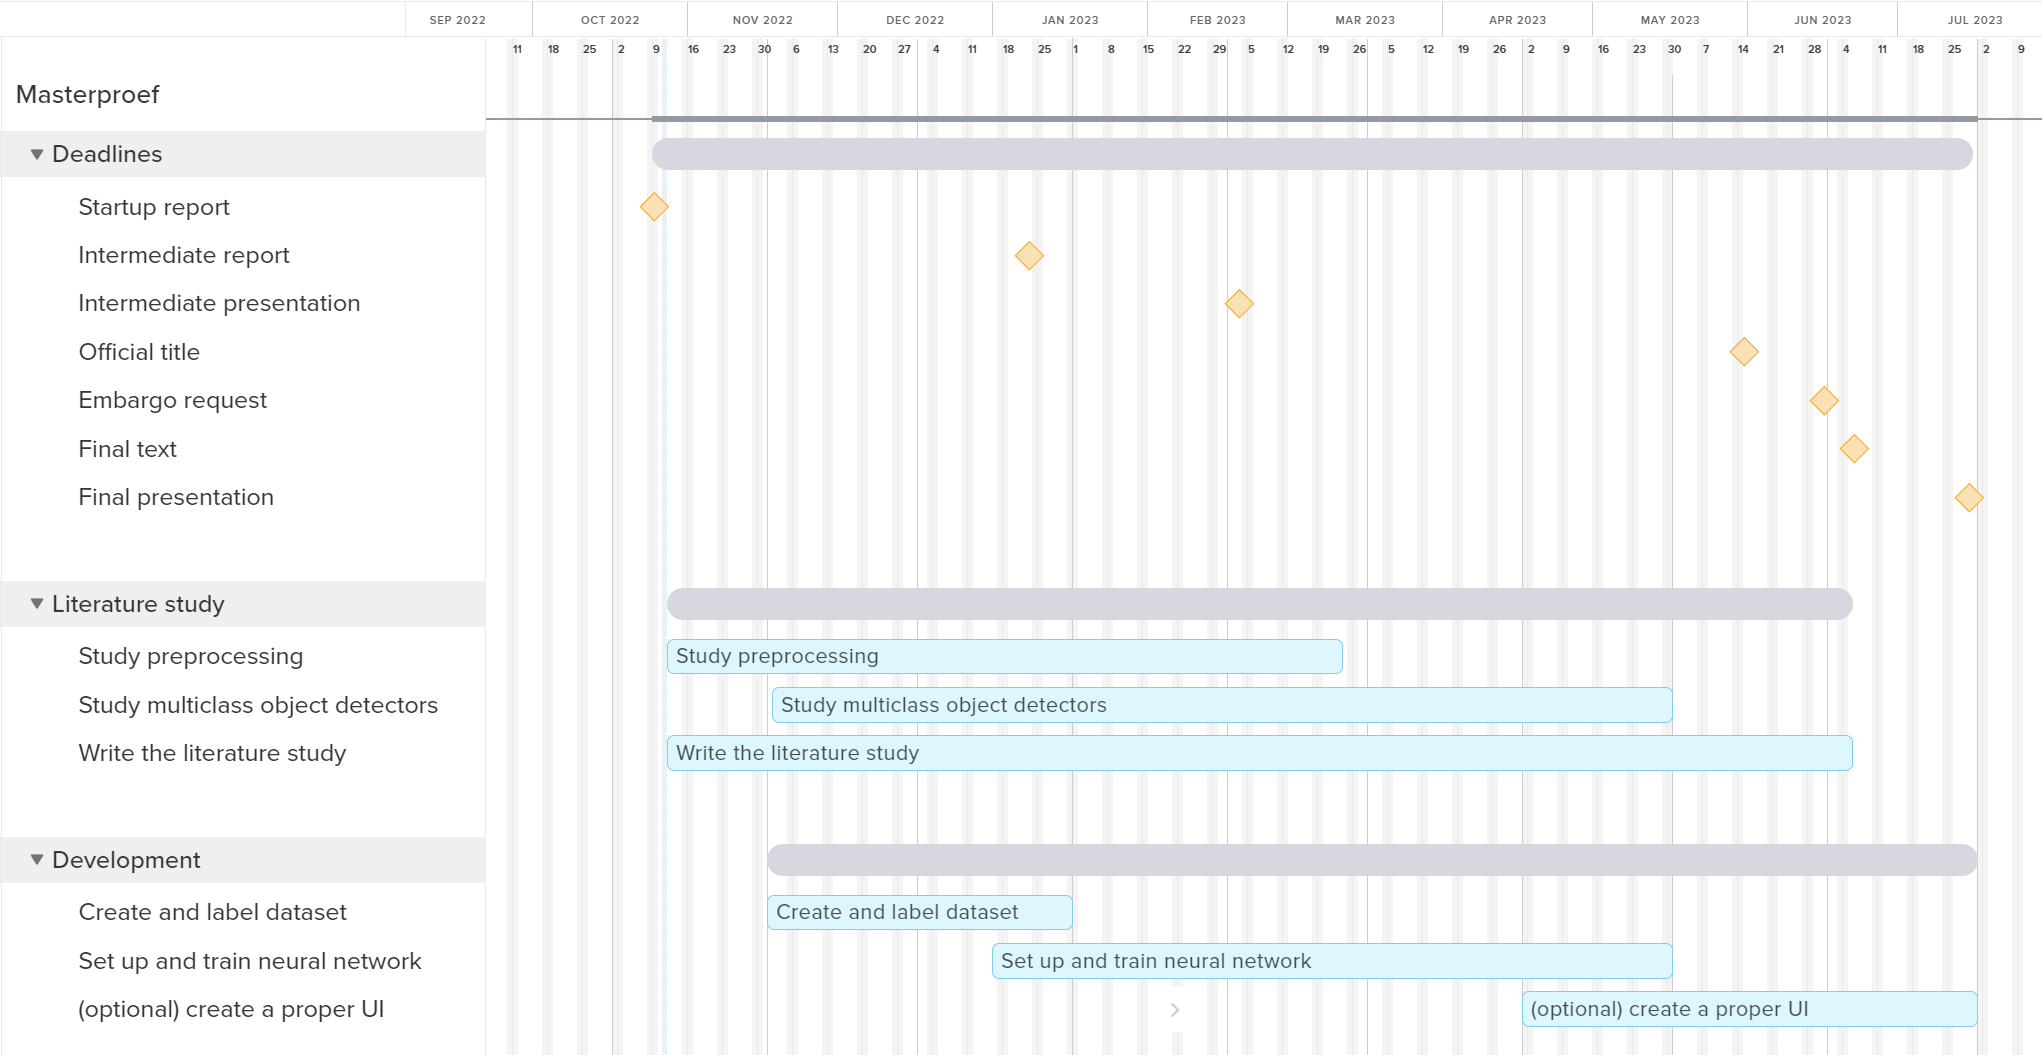
\includegraphics[width=1\linewidth]{gantt.png}
 	\caption{Gantt-chart planning}
   \end{figure}
   As I've only recently changed to this thesis subject there hasn't been any distinctive or notable progress as of now.
   
    
\end{description}


 